
%%This is a very basic article template.
%%There is just one section and two subsections.
\documentclass{scrreprt}
\usepackage{graphicx} 
\usepackage{float}


\linespread{1.4}
%%Variables

\newcommand{\cocos}{cocos2d}
\newcommand{\spriteb}{SpriteBuilder}
\newcommand{\ccscene}{CCScene}


%% Setup code highlighting
\usepackage{listings}
%\usepackage[T1]{fontenc}
%\usepackage[scaled]{beramono}
%\usepackage{tgadventor}
\usepackage[usenames,dvipsnames]{color}
\usepackage[colorlinks=true]{hyperref}

\definecolor{lineno}{rgb}{0.5,0.5,0.5}
\definecolor{code}{rgb}{0,0.1,0.6}
\definecolor{keyword}{rgb}{0.5,0.1,0.1}
\definecolor{titlebox}{rgb}{0.85,0.85,0.85}
\definecolor{download}{rgb}{0.8,0.1,0.5}
\definecolor{title}{rgb}{0.4,0.4,0.4}

\lstset{
    language=Lisp,
    basicstyle=\ttfamily\small\color{code},
    showspaces=false,
    showstringspaces=false,
    numbers=left,
    firstnumber=1,
    stepnumber=5,
    numberfirstline=true,
    numberstyle=\color{lineno}\sffamily\scriptsize,
    keywordstyle=\color{keyword}\bfseries,
    stringstyle=\itshape,
    morekeywords={dosync,if},
    deletekeywords={alter}
}

\makeatletter
\gdef\lst@SkipOrPrintLabel{%
    \ifnum\lst@skipnumbers=\z@
        \global\advance\lst@skipnumbers-\lst@stepnumber\relax
        \lst@PlaceNumber
        \lst@numberfirstlinefalse
    \else
        \lst@ifnumberfirstline
            {\def\thelstnumber{Line \@arabic\c@lstnumber}\lst@PlaceNumber}%
            \lst@numberfirstlinefalse
        \else
            {\def\thelstnumber{-}\lst@PlaceNumber}%
        \fi
    \fi
    \global\advance\lst@skipnumbers\@ne}%
\def\lst@maketitle#1{
   \vskip\abovecaptionskip
   \colorbox{titlebox}{
       \scriptsize
       \color{download}\ttfamily\href{http://example.com/#1}{Download}
       \color{title}\sffamily\bfseries#1}
   \vskip\belowcaptionskip}
\makeatother
%%





\usepackage[framemethod=tikz]{mdframed}
\usetikzlibrary{calc}
\usepackage{kantlipsum}

\usepackage{dingbat}%\eye and \leftpointright

\newcounter{error}[chapter]
\renewcommand*\theerror{\thechapter.\arabic{error}}
\tikzset{
errorsymbol/.style={%
    rectangle,draw=blue,
   ,scale=2,overlay}}

\tikzset{
 lampsymbol/.style={%
   ,scale=2,overlay}}

\newmdenv[hidealllines=true,backgroundcolor=blue!5,%
 frametitle={\stepcounter{error}Comman~Programming~Error~\theerror},
 frametitlefont=\color{blue!80!black}\bfseries,
 skipabove=\topsep,skipbelow=\topsep,nobreak,
 leftmargin=.3cm,rightmargin=.3cm, innerleftmargin=2cm,
 singleextra={\path let \p1=(P), \p2=(O) in ($(\x2,0)+0.5*(2,\y1)$) node[errorsymbol] {\eye};},%
]{error}


\newmdenv[nobreak,middlelinewidth=.8pt,
 frametitlefont=\bfseries,
 leftmargin=.3cm,rightmargin=.3cm, innerleftmargin=2cm,
 skipabove=\topsep,skipbelow=\topsep,
 singleextra={\path let \p1=(P), \p2=(O) in ($(\x2,0)+0.5*(2,\y1)$) node[ lampsymbol] {\leftpointright};
                          \draw[line width=.8pt,white,] ($(O|-P)+(.2cm,0)$) -- ($(P)-(.2cm,0)$); 
                          \draw[line width=.8pt,white,] ($(O)+(.2cm,0)$) -- ($(P|-O)-(.2cm,0)$);
    },%
]{lamp}

\begin{document}

\tableofcontents{}

\chapter{Preample}
Welcome to \textbf{the} most compact yet detailed guide to iOS game programming.
You will be guided through absolutely everything you need to know about
\cocos{} and \spriteb{} and 2d game programming in general.

While we will cover the very basics of game programming, such as scene graphs,
animations and game loops - Objective-C, the language we will be using
throughout the book is not in the scope of things you will learn. When starting
this guide, you are expected to have a solid foundation of Objective-C
knowledge.

The structure in which you will learn is the following:
\begin{itemize}
  \item Tools: Get familiar with the very basics of \cocos{} and \spriteb{}
  \item Infrastructure: Understand that on a high level a game consists of
  scenes. Understand how to create scenes and navigation paths through these
  scenes with \cocos{} and \spriteb{}
  \item Action and Movement: Understand how objects in your game can be moved
  and animated. With \cocos{} and \spriteb{}
  \item Interaction: Understand how user interaction can be captured, including
  Touch interaction and Accelerometer.
  \item Interobject Interaction: Understand how to use the delightfully
  integrated Chipmunk physics engine
  \item Beyond the Basics; Recipes and Best Practices:  Once we have the basics,
  we will look at a ton of recipes and exciting \cocos{} classes, which you can
  use to create any kind of 2d game. Particle Effects, Custom Drawing, Custom
  Shaders, Tile Maps, Networking, Audio, cocos2d UI in depth, etc.
\end{itemize}

\section{Structure of this book}
This book shall function as a learning guide and a reference book. Therefore
most examples will be small and self-contained. Instead of builind a game
throughout the whole book, you will learn by implementing very small projects
that are limited to the material we are currently discussing. 
In my opinion that gives you a better chance of understanding the concepts/code
snippets and using them in your original game, instead starting of from an
example game you have built in this book.

After we have discussed all the basics and you have a good understanding of the
\cocos{} API I will point you to resources that provide example implementations
for specific game types.

There are two different ways to read this book. From the front to the beginning,
gaining knowledge in logical groups. Or if you aren't a beginner and would like
to use this book as an example driven extension of the API reference you can
look up pages by Class names or concept names. There is a special glossar in the
back of this book.

\section{Tools used throughout this book}
The two main tools we will be using are \cocos{} and \spriteb{}. Many of the
problems that occur during game development can be solved by both of these
tools. Wherever possible I will point out both ways, one using only \cocos{} and
one using \spriteb{}. This will allow you to see the advantages of each approach
and finally decide which tool you want to use in certain situations for your own
games.

\chapter{Getting started with \cocos{} 3.0}
\cocos{} is a framework built upon OpenGL ES 2.0. It is designed for 2D games
and abstracts all the complicated rendering work involved in OpenGL programming.
It leaves you behind with a clean and simple API.

If you have never written gaming code before, a few concepts will be new to you.
We will start at the highest level most gaming engines now - the scene graph.

\section{Scene graph in \cocos{} 3.0}
A scene graph is a general computer graphics concept that allows us to
hierarchically organize game objects in a game world. For an example a vehicle can be contained in a game world, a
person can be contained in a vehcile and so forth.
Let's brake this theoretical concept down to \cocos{} terminology. In
\cocos{} we have to key players in our scene graphs: CCScenes and CCNodes. Since
a picture \textit{can} be worth a thousand words, let's start with this diagram:

\begin{figure}[H]
		%\centering
		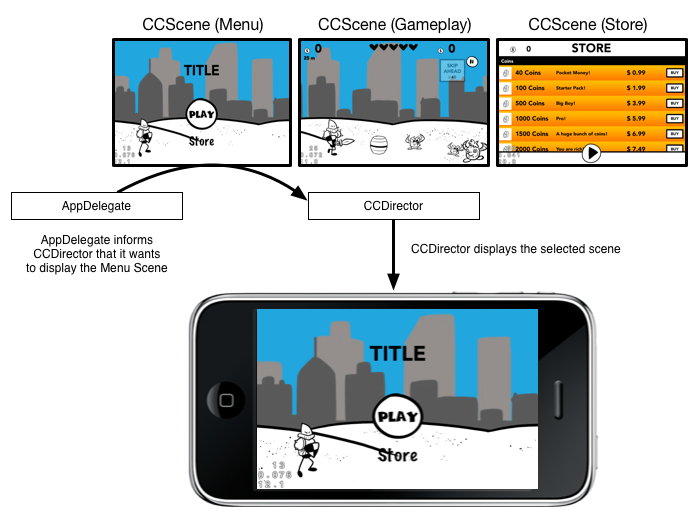
\includegraphics[width=400pt]{images/scenegraph.png}     
		\caption{\textit{Scene graph} in \cocos{}.}
		%\label{labelstruct} 
\end{figure}
 
The diagram represents three different scenes of which each contains
multiple nodes (all buttons, characters, etc. you can see). There are a couple
of takeaways from this diagram:

\begin{itemize}
  \item \textbf{CCDirector} is the highest instance in \cocos{}. It will control
  which scene is presented. You can tell CCDirector to present your main menu,
  your gameplay scene or your highscore scene. CCDirector will allow you to
  present one scene at a time.
  \item \textbf{CCScenes} are used to build a logical group of objects. In
  \cocos{} this almost always means - one scene represents one screen. You will
  have scenes for menues, leaderboards, gameplay, etc. Scenes itself don't have
  a representation, their sole goal is to group CCNodes.
  \item \textbf{CCNodes}. Simply speaking anything that is visible in \cocos{}
  is a subclass of CCNode. We will get to know a diverse range of CCNode
  subclasses very soon, including UI Elements and Sprites\footnote{Sprite
  basically is the game developer word for an image}.
\end{itemize}

The games we write in \cocos{} consist of different scenes. We define the
structure of our game by telling the CCDirector when which scene shall be
presented (menu first, then gameplay, then leaderboard). We create the content
of our scenes using CCNodes.

A CCNode can again contain other CCNodes. We are speaking of a scne graph when
we refer to the strucutre of our CCNodes.

\section{CCNodes in \cocos{} 3.0}
We just learned: \textit{Every visible object in \cocos{} is a subclass of
CCNode}. These are the CCNode subclasses you should know for now:

\begin{description}
  \item[CCSprite] Represents an image or an animated image. Used for characters,
  enemies, etc. in your gameplay.
  \item[CCAnimatedSprite] A convinience class that allows to create animated
  Sprites in just a few lines of code.
  \item[CCNodeColor] A plain colored node.
  \item[CCLabelTTF] A node than represent text in any TTF font.
  \item[CCButton] A interactive node that allows to respond to touch input
  easily.
  \item[CCLayoutBox] A unvisible node that layouts its children.
\end{description}

\section{Let's code}
The easiest way to prove, that \cocos{} is an easy-to-learn, powerful framework
is by starting to write some code. What you have learned so far is enough to
build a simple App with multiple scenes.

Here are the code snippets for the concepts we have already discussed:
\begin{lstlisting}[title=examples/introduction.clj]
[CCDirector sharedDirector]
basically, create a menu scene, create a gameplay scene, add a animated
character to the gameplayscene
\end{lstlisting} 


\begin{error}
Having problems installing \cocos{}? Visit\ldots.
\end{error}

\chapter{Getting started with \spriteb{} 1.0}
Spritebuilder is a tool that derived from Cocosbuilder which originally was
written by Victor Lidholt at Zynga. The goal of Spritebuilder is to provide a
WYSIWYG editor for \cocos{} games. 

In the creation of many scenes you can save a lot of time if you don't
have to layout your menus in code, and instead can place them visually.

If you decide to you use \spriteb{}, you will start your game by creating a new
\spriteb{} project instead of starting of with a Xcode project. Whenever you
start a new \spriteb{} project, it will create and maintain a Xcode project for
you.

Similar to Xcode's Interface Builder you will create interface files using
\spriteb{} and you will be able to connect the interface files with classes you
have created in Xcode.

Interface files in \spriteb{} are called \textit{CCB} files. Each 
CCB file maintains a own scene graph. This means a CCB file can be interpreted
as a CCScene or a CCNode.

If you work on a project using \spriteb{} you workflow will look like this:
\begin{itemize}
  \item Create a project in \spriteb{}
  \item Add images and other resources to your \spriteb{} project.
  \item Create multiple CCB files for the different scenes in your project.
  \item \textbf{Publish} your project in \spriteb{}. This will create or update
  the Xcode project related to your \spriteb{}. 
  \item Add code to you classes in Xcode.
\end{itemize}

Here's a diagram that shows how \spriteb{} and Xcode work together in your
\spriteb{} projects:

\begin{figure}[H]
		\centering
		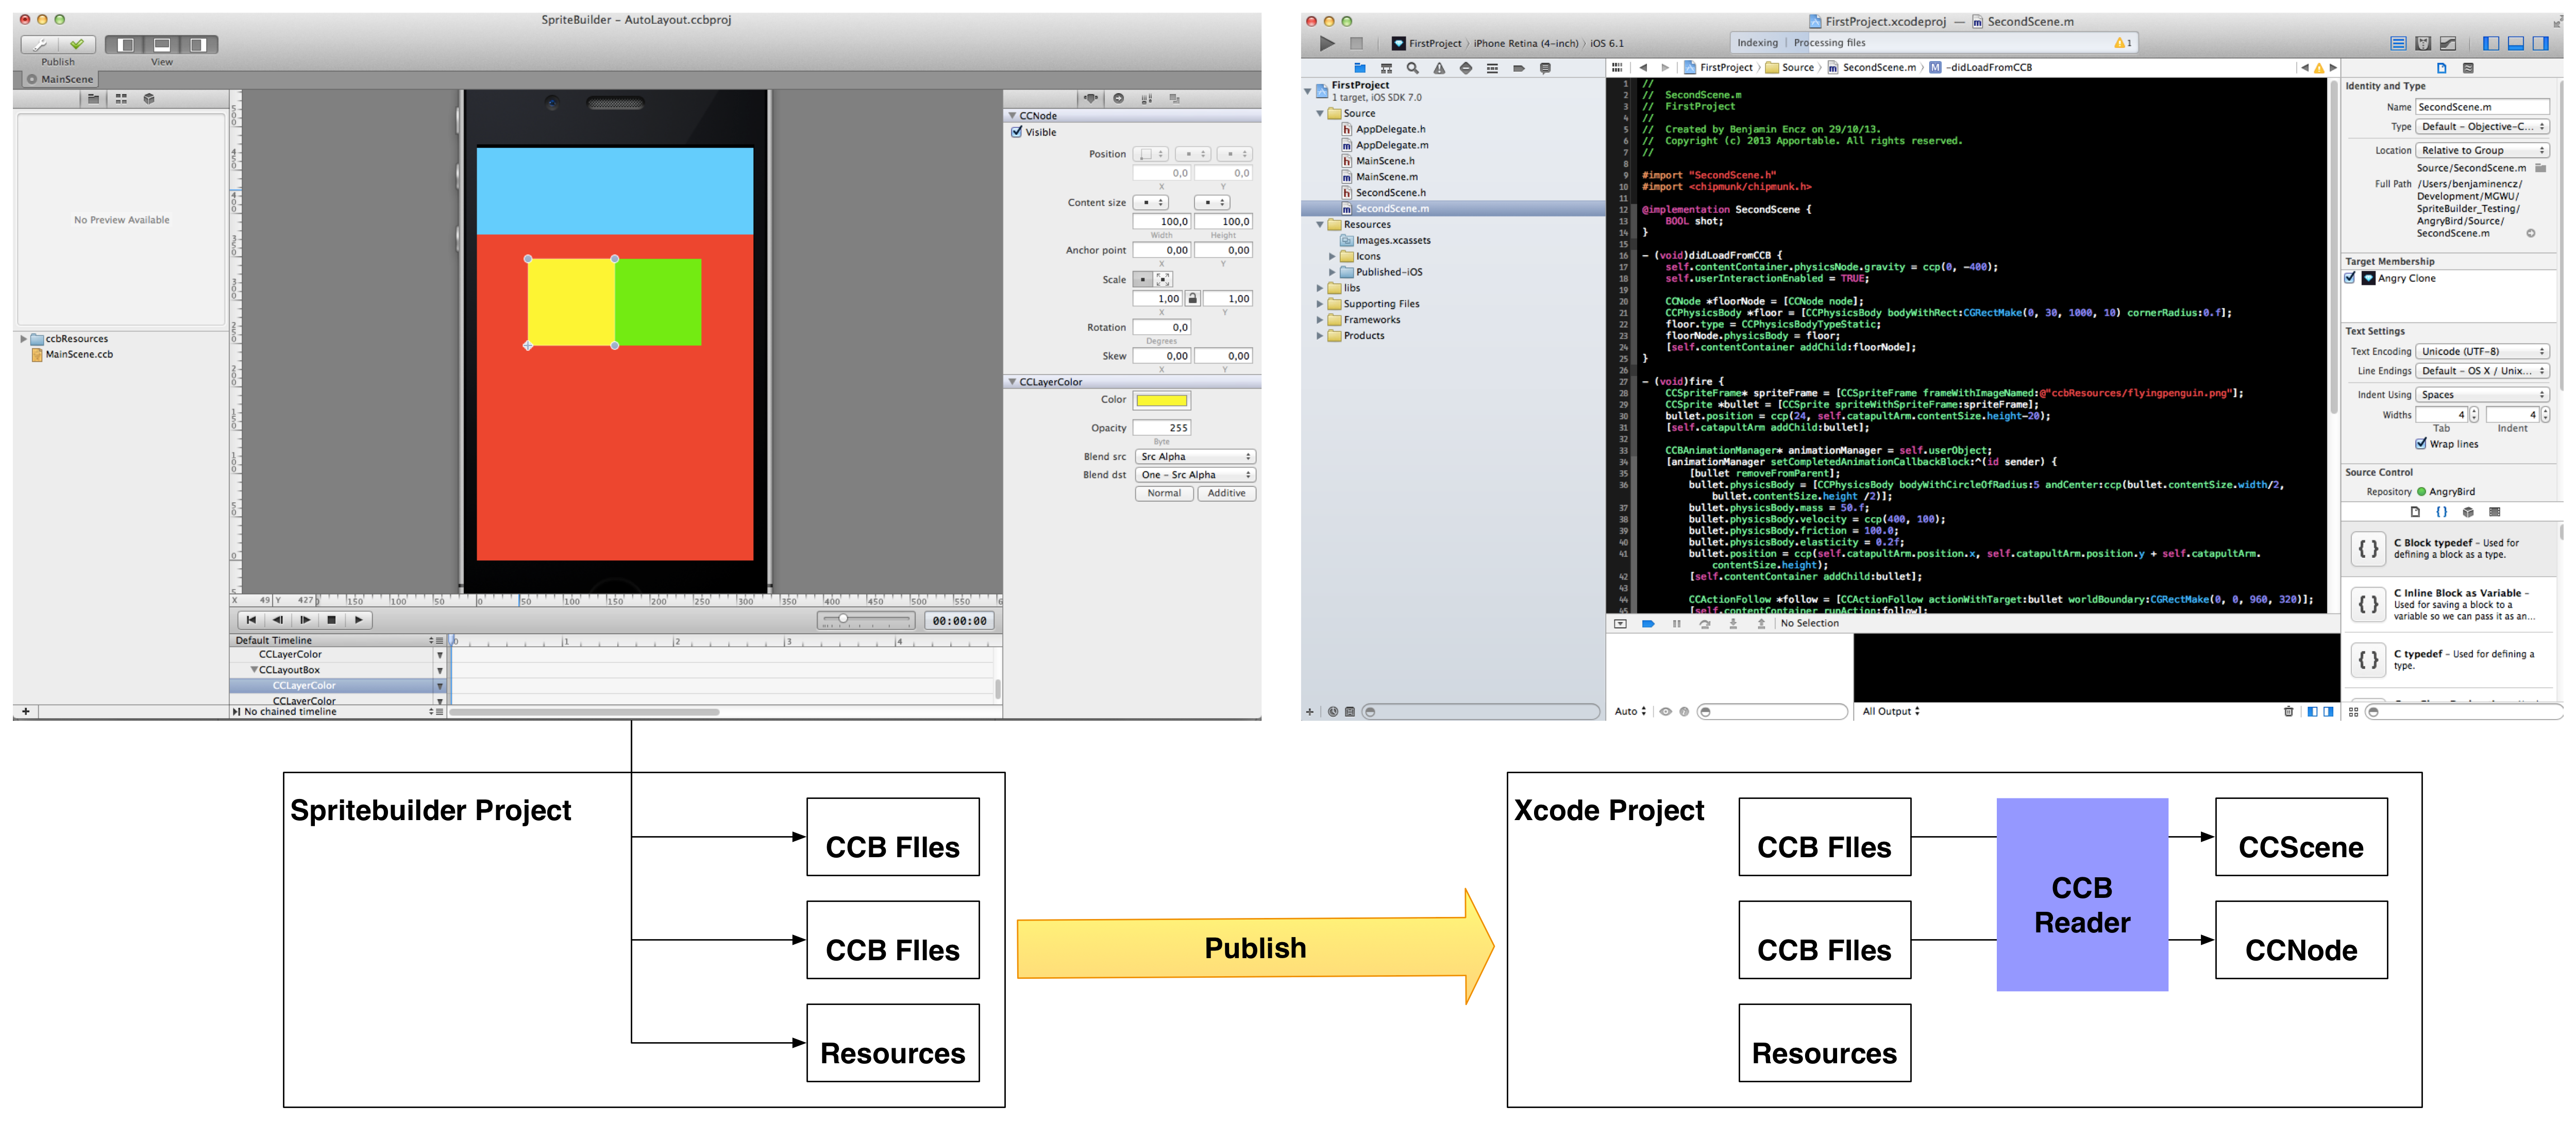
\includegraphics[width=400pt]{images/spritebuilder_publishing.png}     
		\caption{Spritebuilder creates and organizes a Xcode project for you. Adding
		all the resources and scenes you have created.}
		%\label{labelstruct} 
\end{figure}

For those that are interested in a behind the scenes tour, I will give a short
explanation of how \spriteb{} works. In \spriteb{} you create CCB Files, these
store a scene graph; the hierarchy and positions of your nodes. When publishing
in \spriteb the CCB Files and all other resources stored in your \spriteb{}
project are copied to your Xcode project.
When running the project in Xcode a class called CCBReader wil parse your CCB
files and create the according CCNode subclasses to reconstruct the scene graph
you have designed in \spriteb{}.

When you use \spriteb{}, you still implement the navigation in code. The highest
level you will be using CCB files at, are one scene. 
Ok, now let's start by creating our first project using \spriteb{}!

\section{The first Spritebuilder project}
Open \spriteb{} and select \textit{File->New->Project}. Select a folder for your
new project. 

\begin{figure}
		\centering
		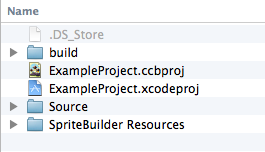
\includegraphics[width=100pt]{images/spritebuilder_project_folderstructure.png}     
		\caption{Typical folder structure after creating a Spritebuilder project. You
		have a \spriteb{} project (.ccbproj)  and a Xcode project (.xcodeproj)}
		%\label{labelstruct} 
\end{figure}

\section{The Spritebuilder User Interface}

\section{Layouting in Spritebuilder}

\chapter{Working with Sprites}
One of the most used classes in your games will be CCSprites. A CCSprite is a
CCNode Subclass that represents an image (for example a game character, a tree,
etc.). 
\section{Getting started with CCSprite}
The easiest way to initialize a sprite it this:
\begin{lstlisting}
-(void)update:(CCTime)delta {
	//implement any custom movement/animation here
}
\end{lstlisting}
\begin{lamp}[frametitle={Optimizing Performance with Batch Nodes}]
Batch Nodes can be used to draw many Sprites witht the same textures at once.
\end{lamp}
\chapter{Animations and Movements}
We have multiple different ways to add activity to scenes in \cocos{}. First, it
is important to know two different forms of activity:
 
\begin{description}
  \item[Movement] If the position of one of our nodes changes over time, we
  consider this a movement.
  \item[Animation] When we iterate through a set of different images, we call
  this an animation.
\end{description}

Let's take a look at movements first.

\section{Implementing Movements}
Since we are using \spriteb{}, we have two different ways to implement this:
In code or through \spriteb{}'s keyframe animations. Implementing physics for
your game is another way to add movement to Nodes, but we are going to spare
that one for later.

\subsection{Implementing Movement manually in code}
We will first try this the hard way - which is always the best way to learn
something new. Since I assume that many readers are new to game development, we
are going to take a small step back and take look at the bigger picture.

One core concept of games is the \textit{game loop}. The game loop takes care of
giving any object in the game, to implement a time based behaviour, by calling
certain methods in a regular interval. In \cocos{} the game loop by itself is
not visible, the only aspect of it we use, is an \textit{update} method. The
update method is called every render cycle. Any CCNode can override this update
method.

This update method is where we can implement any time-based actions. The method
signature looks like this:

\begin{lstlisting}
-(void)update:(CCTime)delta {
	//implement any custom movement/animation here
}
\end{lstlisting}

The one parameter we get passed in is the time that has passed since the update
method has been called last. Whichever action we perform/trigger in the update
method, we need to consider this time factor.

Let's once again implement this by example. We now want to move a simple
unanimated Sprite over the screen with a constant speed:

\begin{lstlisting}
-(void)update:(CCTime)delta {
	//TODO: implement movement code
}
\end{lstlisting}

\subsection{Implementing Movement using CCActions}
When developing games we are mostly confronted with very similar problem sets.
\cocos{} provides a lot of functionality for common use cases. One of these
convinience concepts are \textit{CCActions}. CCNodes can run CCActions. The
CCActions a CCNode runs can affect different properties of the CCNode such as
position, color or scale.

So for the use case we have seen above, moving a sprite across the screen, we
don't need to implement custom movement code, we can use CCActions.

There are a large amount of CCAction types in \cocos{}:
\begin{description}
  \item[CCActionMove] ...
\end{description}

We will first take a look at how we can implement the movement using a
CCActionMove, then we will take a clooser look at the other CCAction types and
how and when they can be used.

Actually, implementing this is amazingly easy. We create a CCActionMove and let
our CCNode run this action:
\begin{lstlisting}
	CCActionMove *move = [CCActionMove actionWithTargetPosition:pos duration:1.f];
	[ship runAction:move];
}
\end{lstlisting}

\subsection{Implementing Movement with \spriteb{}}

\section{Implementing Animations}
This section will have to challenges. First we will need to learn a new tool, to
create images in a way, that we can use them for sprite animations. Second we
will learn how to implement these animations in code and in \spriteb{}.

In \cocos{}, as in many 2D game engines, animations consist of a group of
frames. For example a running animation will be a set of 5 different pictures
showing a character in 5 different stages of a running movement. Basically all a
game has to do is to switch between these 5 different images with a certain
delay that makes the animation believable. This is the same approach as used by
GIF-File animations (these things that splattered the first generation of the
internet).

\section{Creating an animation Spritesheet}
\section{Implementing animations in code}
\subsection{Implementing an animation using CCActions}
\subsection{Implementing an animation using a convenience class}
\section{Implementing animations using \spriteb{}}

\chapter{User Interaction}
User Interaction is another important foundation for any game. This chapter
concludes the minimum basic understanding you need to build an actual game - and
we have a lot to discuss.

New input capabilities have revolutionized the gaming experience on mobile
devices and have created completely new genres of games. In order to create
great mobile games you need to be able to work with all the possible input types
modern iOS devices provide:
\begin{itemize}
  \item Touch Input
  \item Accelerometer Input
  \item Gesture Recognition
\end{itemize}
We will start looking at simple touch input first, since this is the easiest and
most used control scheme in games.
\section{Handling touch input in \cocos{}}
\section{Handling Gestures in \cocos{}}
\section{Handling Accelerometer input in \cocos{}}

\chapter{User Interfaces in \cocos{}}
Similar to UIKit, \cocos{} provides a set of UI components you should be
familiar with:
\begin{itemize}
  \item CCButton
  \item CCTextField
  \item CCTableView
\end{itemize}

\section{Positioning and Layouting in \cocos{}}
We will first look at positioning: a Node is placed at a certain positioning.
After that we will take a look at layouting: a Node's position is determined by
a layouting mechanism.
\subsection{Positioning}
In order to create your first menu in \cocos{} you need to understand how the
layouting/positioning within CCScenes works. If you are already
familiar with UIKit (Apple's Framework to build iOS Apps with the native
interface components) there is one significant difference: \cocos{}'s root point
(x=0, y=0) is in the bottom left corner.

Another aspect to positioning which isn't used by many other frameworks
are anchor points. Anchor points define which position within your Node is used
to place the Node. Most Node's anchor point default to 0,0 (the bottom left
corner), while some CCNode subclasses, such as CCSprite override this property.
CCSprite's anchor point defaults to (0.5, 0.5) the middle of itself.
Changing the anchor point will affect positioning and rotation of your Nodes.

\cocos{} 3.0 also introduces a new concept called \textit{positioning types}.
These positioning types influence the way, the position property of your Node is
interpreted. Here an overview of the available position types:

\begin{description}
  \item[CCNormalizedPosition] Normalized means that the position is expressed
  relative to the parents content size. A 0.5 value for the x-Position means,
  that the Node will be placed at 50 percent of the parents width - thus
  horizontally centered.
  \item[CCAbsolutePosition] Default. Interpretes the position as absolute
  position.
\end{description}

Let's come up with some layouting examples to make these theoretical terms into
practical code:

\begin{lstlisting}
/* position CCNode at top right; There are other solutions, but this is the
ideal one:*/
CCNode *node = [CCNode node];
node.anchorPoint = (1.f, 1.f)
node.positioningType = CCTypeNormalized;
node.position = (1.f,1.f);

/* Place this in the center:*/ 
CCNode *node = [CCNode node];
node.anchorPoint = (0.5f, 0.5f)
node.positioningType = CCTypeNormalized;
node.position = (0.5f,0.5f);
\end{lstlisting}

Positioning types can also be combined. Assume we want to center an element
horizontally, but want it's vertical position to be 100 points from the top of
the screen. This means we'd like normalized position for our x positioning, but
absolute positioning for our y position:

\begin{lstlisting}
/* position CCNode at top right; There are other solutions, but this is the
ideal one:*/
CCNode *node = [CCNode node];
node.anchorPoint = (0.5f, 1.f)
node.positioningType = CCPositionTypeMake(CCTypeNormalized, CCTypeAbsolute);
node.position = (0.5f,parent.contentSize.height - 100);
\end{lstlisting}
 
\subsection{Layouting}
CCLayoutBox has already been mentioned as one of the important CCNode types in
\cocos{}. CCLayoutBox can take care of automatically positioning your nodes, by
aligning them vertically or horizontally with a margin between the items that
can be defined manually.

Here's a short example:
\begin{lstlisting}
/* TODO: layout box example code */
CCLayoutBox *layoutBox = [CCLayoutBox layoutBox];
\end{lstlisting}
 

\chapter{Physics}
This may seem sarcastic, but we are going to start this chapter with thinking
about how we can avoid using physics in our games - some games simply do not
need physics calculations and can work with CCActions and simple collision
detection instead - potentially making the game developers life a lot easier.

\chapter{Particle Effects}
Particle Effects are the secret sauce to the graphics of your 2d game. They can
make graphics a lot more enjoyable. You now will learn how to create particle
effects in code and using Spritebuilder. However, before we discuss how to
create particle effects we need to understand which art is required for particle
effects.

\section{Art for particle effects}
Basically a particle effect (in \cocos{}) consists of a huge amount of Sprites
which are colored/blurred, or otherwise graphically manipulated, and moving in
patterns. This means the basic element of every particle effect is a texture for
a single particle. You can download the texture for our firt particle effect
here:TODO downloadlink. Two important things to note: the texture has a
transparent background and its structure is colored in grayscale colors. This
way the particle can be blended into any color. 
 \begin{figure}[H]
		\centering
		
\includegraphics[width=80pt]{images/particle_stars.png}     
		\caption{A classic texture for a particle effect.}
\end{figure}

\section{Particle Effect Basics}
\cocos{} provides a convinience class that allows to create particle effects
with a wide variety of parameters: CCParticleSystem.
In the appendix you can find a table that provides a brief description of each
parameter. However, it is a lot easiert to start with some examples.
\section{Particle Effects in \cocos{}}
In case you are not using Spritebuilder for your game - or you just want to
learn the underlying basics of creating custom particle effects, this chapter is
for you. We will learn how to build particle effects in code and using the
popular tool \textit{Particle Designer}.
\begin{lamp}[frametitle={Following this tutorial}]
If you want to implement this tutorial you need to start with this template
project: .We will add multiple scenes for different applications of particle
effects.
\end{lamp}
\subsection{Configuring particle effects in code}
Most of the time you will want to design particle effects in a graphical editor
that provides a nice visual preview. However, to understand the basics we will
create our first particle effect in code (this is a great example from 
the cocos2d tests).

The steps we need to perform:
 \begin{itemize}
   \item create a CCParticleSystem
   \item select a particle texture
   \item set a duration for the particle effect
   \item set a huge amount of further, optional parameters
 \end{itemize}
\textbf{Now let's create our first particle effect.}
Add a new scene called \textit{ParticleEffectScene} to your project. You also
need to add a button to the \textit{MenuScene} that will allow us to present the
new \textit{ParticleEffectScene}.  
I won't provide the complete setup code (it's mostly
boring but can be found here: https://gist.github.com/Ben-G/8340545), here's the relevant part:
\begin{lstlisting}
    CCParticleSystem *emitter = [[CCParticleSystem alloc] initWithTotalParticles:50];
    emitter.texture = [[CCTextureCache sharedTextureCache] addImage: @"stars-grayscale.png"];
	emitter.duration = CCParticleSystemDurationInfinity;
    // lots of further parameters
\end{lstlisting}
Once the particle system is created, you add it as a child to your scene:
\begin{lstlisting}
    emitter.positionType = CCPositionTypeNormalized;
    codeParticleEffect.position = ccp(0.5f, 0.5f);
    [self addChild:emitter];
\end{lstlisting}
There is no need to start the particle effect - it is started as soon as it is
added to a parent node. However you can manually start/stop a particle system by
using the \textit{stopSystem} and \textit{resetSystem} methods. Now you can run
the app and you should see a particle effect in the middle of the scene. (TODO:
add screenshot) 
\subsection{Particle Effects with plists}
If you took some time to read through the setup in code
(https://gist.github.com/Ben-G/8340545) you have seen that it is very cumbersome
and nothing that actually should be part of your code base. Luckily \cocos{}
allows us to read particle effects from plist-files. You can fill these plists
manually, using the same parameters as when setting up particle systems in code
- however, the value of using plists only fully unfolds when you use graphical
editors to create your particle effects. Spritebuilder comes with an integrated
particle effect designer. If you don't use Spritebuilder, \textit{Particle
Designer}(http://particledesigner.71squared.com/) is the preferred tool to
create particle effects.
\subsection{Particle Effects in Particle Designer}
\subsection{Including particle effects in your gameplay}
Now that we have the basics it's the right time to add some best practices.
Mostly you will want to add particle effects dynamically to your scenes, based
on certain events such as collisions or explosions. Let's create a new class
called \textit{ParticleGamePlayScene}, again, don't forget to add a entry to
\textit{MenuScene} that let's you push the new scene.
We're going to build following scene:
 \begin{itemize}
   \item two spaceships, one at the left and one at the right edge of the sceen
   \item when a ship get's touched it fires a bullet at the other ship
   \item when a bullet hits another ship we play a small explosion particle
   effect
   \item when a ship got hit three times it explodes, we play a large explosion
   particle effect and remove the ship from the scene 
\end{itemize}
 
\section{Particle Effects in Spritebuilder}
Now you will learn how to add particle effects to your Spritebuilder project.
First open the menu to add a new interface file: 
\begin{figure}[H]
		\centering
		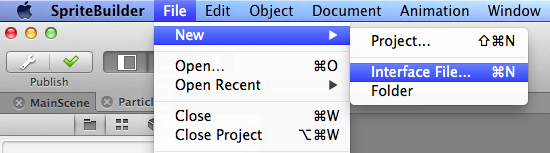
\includegraphics[width=275pt]{images/particles/Spritebuilder_ParticleEffect_Menu1.png}   
\end{figure}
Next, select \textit{Particles} as document type:
\begin{figure}[H]
		\centering
		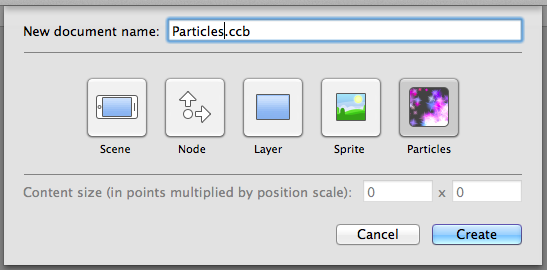
\includegraphics[width=275pt]{images/particles/Spritebuilder_ParticleEffect_Menu2.png}   
\end{figure}
Now you should see the newly created particle effect on your stage. To select
the node you can use the timeline and select the \textit{CCParticleSystemQuad}
(highlighted blue in the screenshot):
\begin{figure}[H]
		\centering
		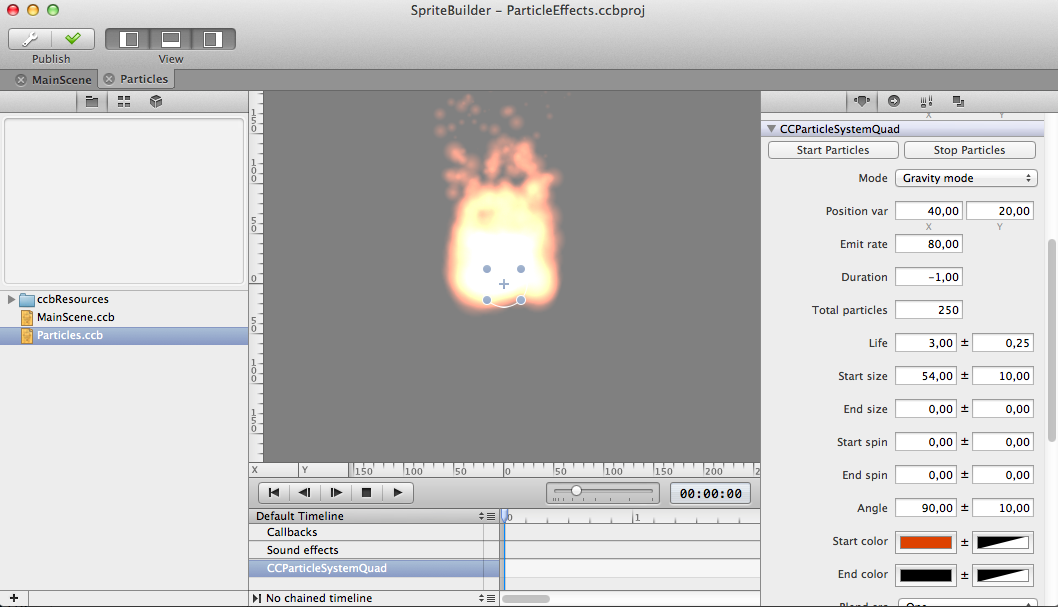
\includegraphics[width=375pt]{images/particles/Spritebuilder_ParticleEffect_CCB.png}   
		\caption{Stage with a default particle effect}
\end{figure}
In the inspector on the right you can see all (check if this is true) properties
that we have set in code previously. You can update them and get a live preview
of how they influence your particle effect. 

Spritebuilder comes with a nice library of template particle effects. You can
view them in the rightmost tab of the inspector:
\begin{figure}[H]
		\centering
		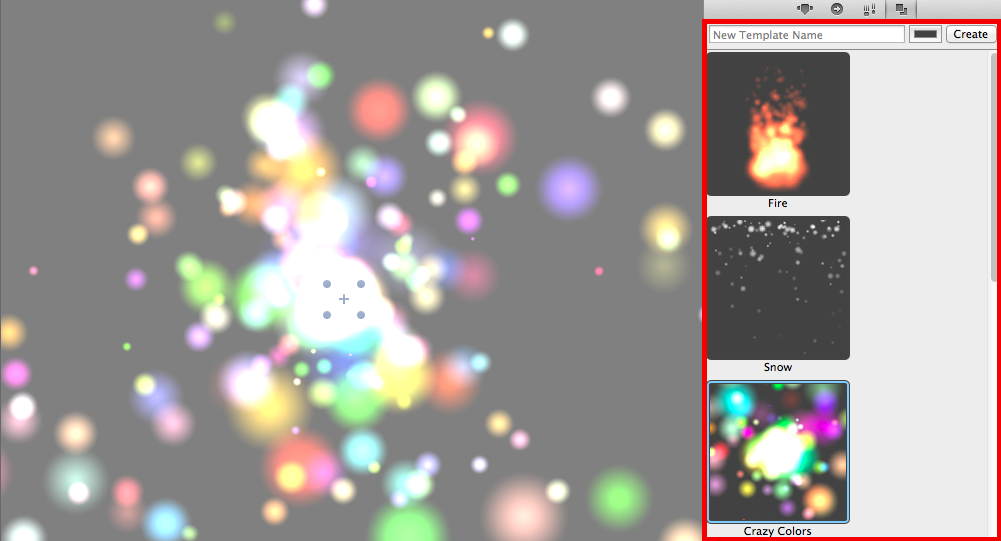
\includegraphics[width=375pt]{images/particles/Spritebuilder_ParticleEffect_Templates.png}   
		\caption{Spritebuilder provides many particle effect templates}
\end{figure}
to select one of the templates, simply double-click it.
\subsection{Adding the particle effect to your scene}
Spritebuilder creates a new CCB File for each of your particle effects. If you
want to add a particle effect to one of your gameplay scenes you need to add the
CCB File of the particle effect as a child. 
You can do this by dropping a \textit{Interface File} child node on your target
scene:
\begin{figure}[H]
		\centering
		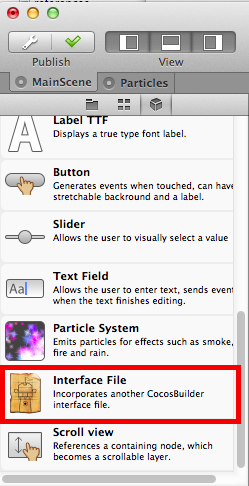
\includegraphics[width=70pt]{images/particles/Spritebuilder_ParticleEffect_AddInterfaceFile.png}   
		\caption{Interface Files let you include CCB Files in other CCB Files}
\end{figure}
Once the \textit{Interface File} node is added, you can choose which CCB File
shall be included. The inspector provides a dropdown with all available CCB
Files, here you can choose the CCB of your particle effect.
 \begin{figure}[H]
		\centering
		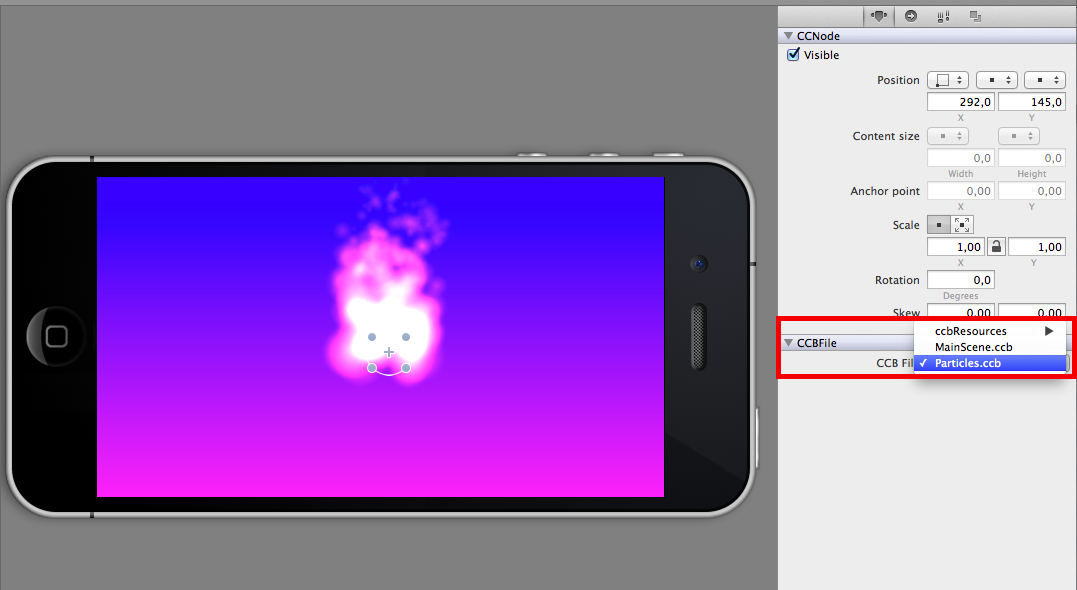
\includegraphics[width=375pt]{images/particles/Spritebuilder_ParticleEffect_InterfaceFile.png}
		\caption{In the dropdown of the inspector you can choose which CCB File
		should be included}
\end{figure}
Now you have succesfully added the particle effect to your scene. However,
mostly when you work with particle effects you will not add to your scene
statically, as we just did, but you will want them to appear when certain events
occur, e.g. collisions or explosions. In the next chapter we will take a look
how we can add particle effects to our gameplay - dynamically. 
\subsection{Including particle effects in your gameplay}
 

\chapter{Audio}

\chapter{Tilemaps}

\chapter{Appendix A: Writing your own SpriteBuilder Plugins}
\chapter{Appendix B: Particle Parameters}
\begin{table}
    \begin{tabular}{lll}
    Mode                     & Parameter               & Description \\
    Gravity Mode (Mode A)    & ~                       & ~           \\ \hline
    ~                        & Gravity                 & a           \\
    ~                        & Direction               & a           \\
    ~                        & Speed                   & a           \\
    ~                        & Tangential acceleration & a           \\
    ~                        & Radial acceleration     & ~           \\
    Radius Mode (Mode B)     & ~                       & ~           \\
    ~                        & Start Radius            & a           \\
    ~                        & End Radius              & a           \\
    ~                        & Rotate                  & a           \\
    Properties for all Modes & ~                       & ~           \\
    ~                        & Life                    & a           \\
    ~                        & Start spin              & a           \\
    ~                        & End spin                & a           \\
    ~                        & Start size              & a           \\
    ~                        & End size                & a           \\
    ~                        & Start color             & a           \\
    ~                        & End color               & a           \\
    ~                        & Life                    & a           \\
    ~                        & Blending function       & a           \\
    \end{tabular}
\end{table}
\end{document}
